% Created 2022-09-30 Fri 16:24
\documentclass[9pt, b5paper]{article}
\usepackage{xeCJK}
\usepackage{minted}
\usepackage[T1]{fontenc}
\usepackage[scaled]{beraserif}
\usepackage[scaled]{berasans}
\usepackage[scaled]{beramono}
\usepackage{graphicx}
\usepackage{xcolor}
\usepackage{multirow}
\usepackage{multicol}
\usepackage{float}
\usepackage{textcomp}
\usepackage{algorithm}
\usepackage{algorithmic}
\usepackage{latexsym}
\usepackage{natbib}
\usepackage{geometry}
\geometry{left=1.2cm,right=1.2cm,top=1.5cm,bottom=1.2cm}
\newminted{common-lisp}{fontsize=\footnotesize} 
\usepackage[xetex,colorlinks=true,CJKbookmarks=true,linkcolor=blue,urlcolor=blue,menucolor=blue]{hyperref}
\author{deepwaterooo}
\date{\today}
\title{Unity Android SDK/NDK 俄罗斯方块砖3D小游戏}
\hypersetup{
  pdfkeywords={},
  pdfsubject={},
  pdfcreator={Emacs 27.1 (Org mode 8.2.7c)}}
\begin{document}

\maketitle
\tableofcontents


\section{游戏基础框架的快速链接}
\label{sec-1}
\begin{itemize}
\item 将游戏的绝大部分逻辑放到热更新程序包下执行,以便实现随时热更;
\item 暂时不考虑服务器,所以先弄个本地服务器试运行着
\item 把基本的unity游戏逻辑与ILRuntime + MVVM的唯一一个(如果我需要多个场景,那么我需要添加很多场景切换的逻辑,所以最简单的办法就是游戏自始自终只使用一个场景,其它所有变更的都只是Panel View UI。)场景试着尽快运行起来
\item 打包第一个场景: 好像是两个前后相差几个的游戏引擎不太兼容,打包的预设不识别,会再看一看(先粗糙地封了一整个场景,会把可能热更新的折下来折小一点儿,晚些时候)
\end{itemize}

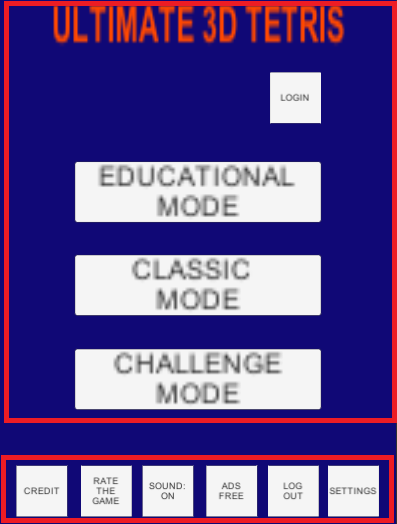
\includegraphics[width=.9\linewidth]{./pic/readme_20220929_220207.png}
\begin{itemize}
\item 
\item 
\end{itemize}
\section{把原理弄懂}
\label{sec-2}
\begin{itemize}
\item 热更新模块的实现:以前的设计模式和实现的功能还是比较完整的;现在更成熟一点儿,需要把热更新模块补充出来;
\item ILRuntime + MVVM框架设计:两者结合,前几年的时候没能把MVVM理解透彻;
\item 上次前几年主要的难点:好像是在把MVVM双向数据绑定理解得不透彻;那么这次应该就狠没有问题了,更该寻求更好的设计与解决方案;服务器方面的知识点相对欠缺
\item 下面有个狠好玩的图: 它描述了应用从店里下载安装后,热更新资源上载到服务器以及客户端检查更新,下载实现更新的大致过程。
\end{itemize}

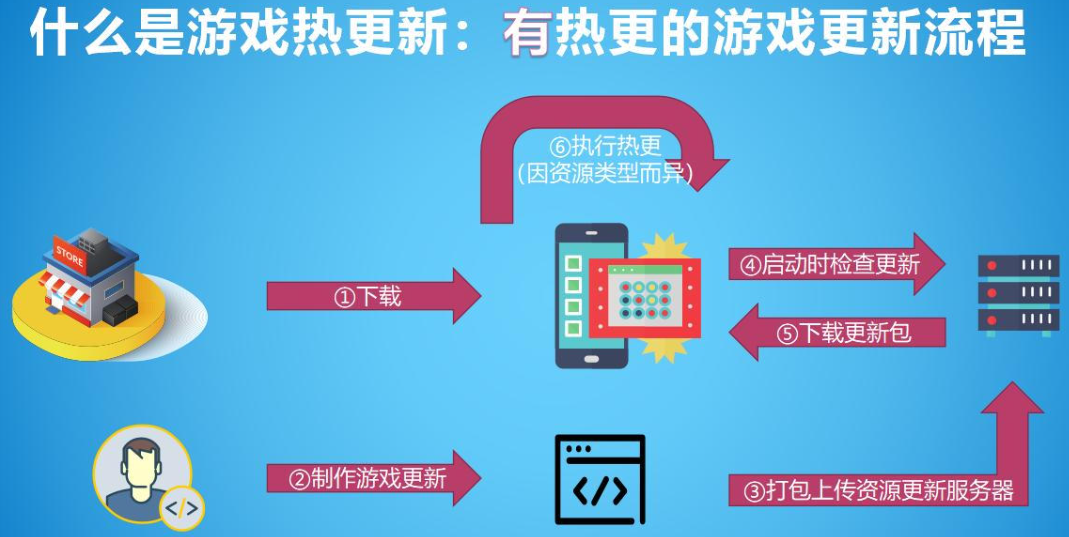
\includegraphics[width=.9\linewidth]{./pic/readme_20220930_162306.png}

\begin{itemize}
\item 资源包的准备:热更新分程序热更新和资源的热更新;那么现在的项目就是资源的热更新是分成了两个小项目来实现资源热更新资源包的自动打包(分场景打包和其它资源打包);程序热更新因为主要是更新视图,游戏的所有基本逻辑主程序都运行在热更新程序包下,所以三个小项目便可以实现所有资源(是指包括资源和程序)的自动打包为可上载热更新服务器的程序包。(三个小项目看起来是最简单的,但是全部实现出来可能还是工作量最大的)
\item 服务器层的相对理解:应该是需要一个好用的第三方程序,或是合适好有物服务器来提供必要的资源包上载到服务器;服务器层可能还需要根据不同的应用平台(IOS安卓等)来进行一定的配置,以及必要的压力测试保证相对大量用户的情况下可以正常上载下载运行(后一步暂不考虑)
\item 客户端:对于不同的客户端应用平台,游戏运行时的资源包MD5比对的原理要再熟悉一下
\item 我觉得我该考虑尽快至少建个本地服务器了
\item 性能优化:另外是对其实高级开发的越来越熟悉,希望应用的性能表现,尤其是渲染性能与速度等、这些更为高级和深入的特性成为这次二次开发的重点。

\item 现在是把自己几年前的写的游戏全忘记了,需要回去把自己的源码找出来,再读一读熟悉一下自己的源码,了解当时设计的估缺点,由此改进更将
\end{itemize}

\section{几种不同热更新模式的探讨}
\label{sec-3}
\subsection{HybridCLR——划时代的Unity原生C\#热更新技术: IL2CPP与热更新}
\label{sec-3-1}

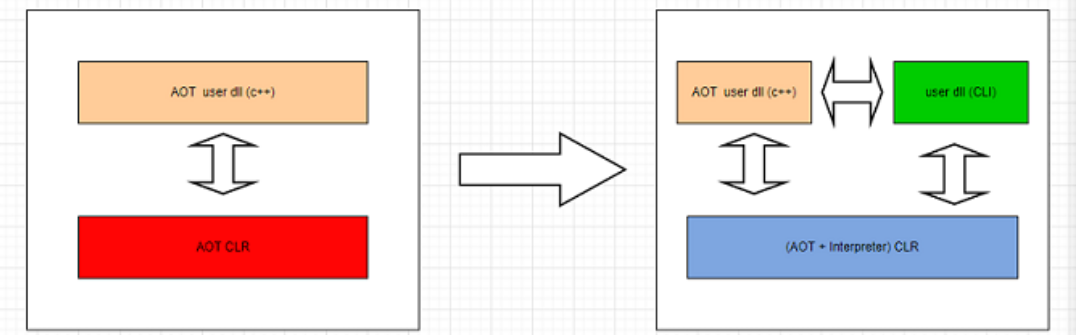
\includegraphics[width=.9\linewidth]{./pic/readme_20220930_082537.png}
很不幸,不像Mono有Hybrid mode execUtion,可支持动态加载DLL。IL2CPP是一个纯静态的AOT运行时,不支持运行时加载DLL,因此不支持热更新。
目前unity平台的主流热更新方案xLUa、ILRUntime之类都是引入一个第三方VM(VirtUal Machine),在VM中解释执行代码,来实现热更新。这里我们只分析使用C\#为开发语言的热更新方案。这些热更新方案的VM与IL2CPP是独立的,意味着它们的元数据系统是不相通的,在热更新里新增一个类型是无法被IL2CPP所识别的(例如,通过System.Activator.CreateInstance是不可能创建出这个热更新类型的实例),这种看起来像,但实际上又不是的伪CLR虚拟机,在与IL2CPP这种复杂的CLR运行时交互时,会产生极大量的兼容性问题,另外还有严重的性能问题。
一个大胆的想法是,是否有可能对IL2CPP运行时进行扩充,添加Interpreter模块,进而实现Mono hybrid mode execUtion这样机制?这样一来就能彻底支持热更新,并且兼容性极佳。对开发者来说,除了解释模式运行的部分执行得比较慢,其他方面跟标准的运行时没有区别。
对IL2CPP加以了解并且深思熟虑后的答案是——确实是可行的!具体分析参见第二节《关于HybridCLR可行性的思维实验》 。这个想法诞生了HybridCLR,unity平台第一个支持iOS的跨平台原生C\#热更新方案!
\begin{itemize}
\item 现在也简单地理解一下这个方案最简单原始案例实现的基本原理,若有兴趣,就可以再深入地探讨一下
\end{itemize}


\section{环境弄得比较好的包括:}
\label{sec-4}
\begin{itemize}
\item 电脑的配置有限,文件稍微大一点儿的时候已经不太好处理了;所以不得不分割成多个小文件
\item 几年过去了,ILRuntime已经不是最新最前沿的热更新技术,成为别人更新技术的一个子模块,所以还是自己再搜索找一下有没有更方便的热更新实现方法(若是不得,我就在自己游戏里实现 ILRuntime + MVVM实现视图等的更新)
\end{itemize}
- 这一两天作必要的文献研究,确定哪个大的模块版块需要实现或是修改优化,列个大致计划,把它们一一完成;希望截止这个周末周六周日能够把这个部分确定得相对精确
\begin{itemize}
\item 小笔记本电脑太慢了,会回家再读其它模块的源码,理解透彻。爱表哥,爱生活!!
\item 输入法的搭建:终于用到了自己之前用过的好用的输入法
\item 这两天开车疲累,最迟明天中午会去南湾找房间出租,尽快解决搬家的问题;昨天晚上回来得太晚了,一路辛苦,路上只差睡着,回到家里补觉补了好多个小时。
\item 小电脑,笔记本电脑里的游戏环境搭建,今天下午去图书馆里弄(今天下午去图书馆里把需要借助快速网络来完成的事情都搭建好;家里被恶房东故意整了个腾腾慢的网,故意阻碍别人的发展,谁还愿意再这样的环境中继续住下去呢?!!!)
\end{itemize}
- 能够把程序源码读得比较懂,也并不代表把所有相关的原理就全部弄懂了;不是说还有多在的挑战,而是说要不断寻找更为有效的学习方法,快速掌握所有涉及到的相关原理;在理解得更为深入掌握了基本原理的基础上再去读源码,会不会更为有效事半功倍呢?这是一颗永远不屈服的心,爱表哥,爱生活!!!
\section{ILRuntime 库的系统再深入理解}
\label{sec-5}
\subsection{ILRuntime基本原理}
\label{sec-5-1}
\begin{itemize}
\item ILRuntime借助Mono.Cecil库来读取DLL的PE信息,以及当中类型的所有信息,最终得到方法的IL汇编码,然后通过内置的IL解译执行虚拟机来执行DLL中的代码。IL解释器代码在ILIntepreter.cs,通过Opcode来逐语句执行机器码,解释器的代码有四千多行。
\end{itemize}

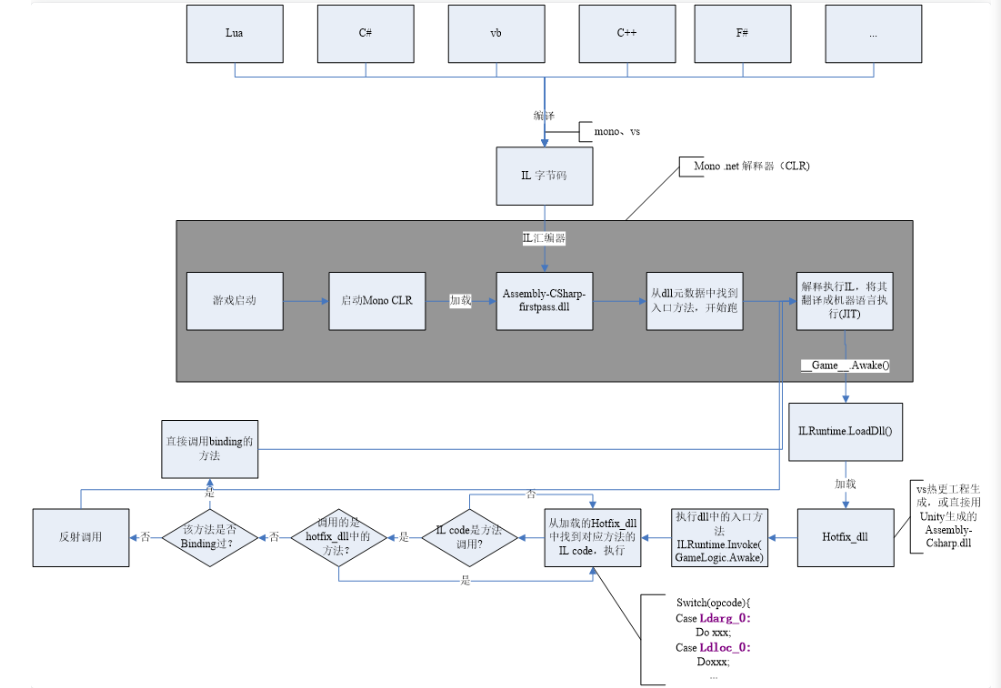
\includegraphics[width=.9\linewidth]{./pic/readme_20220926_094936.png}

\subsection{ILRuntime热更流程}
\label{sec-5-2}

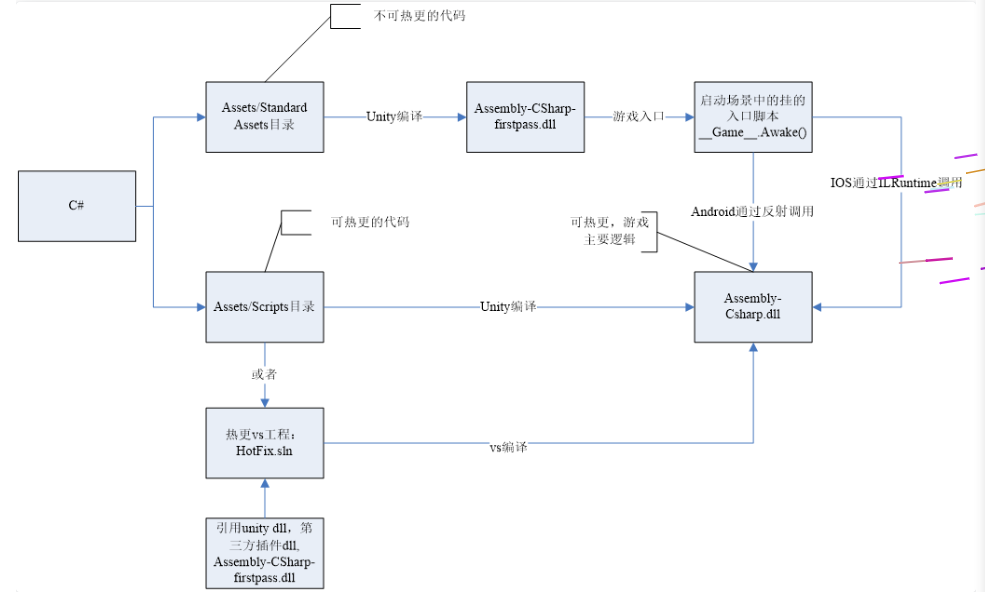
\includegraphics[width=.9\linewidth]{./pic/readme_20220926_095022.png}
\subsection{ILRuntime主要限制}
\label{sec-5-3}

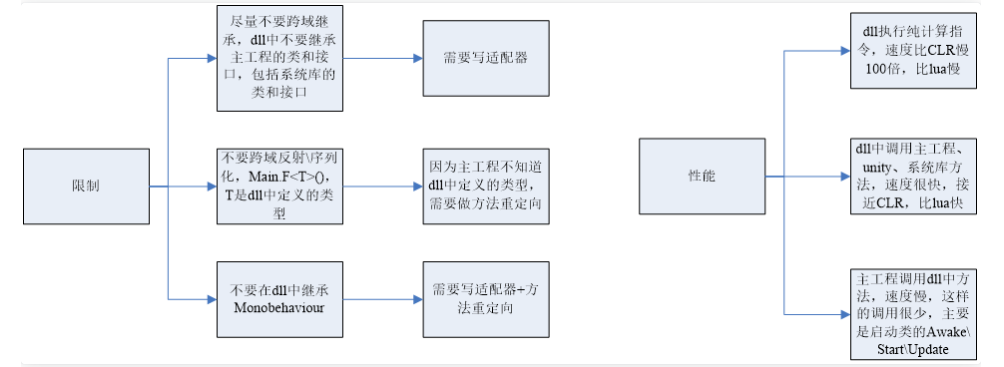
\includegraphics[width=.9\linewidth]{./pic/readme_20220926_095555.png}
\begin{itemize}
\item \textbf{委托适配器(DelegateAdapter)} :将委托实例传出给ILRuntime外部使用,将其转换成CLR委托实例。
\end{itemize}
由于IL2CPP之类的AOT编译技术无法在运行时生成新的类型,所以在创建委托实例的时候ILRuntime选择了显式注册的方式,以保证问题不被隐藏到上线后才发现。
\begin{minted}[fontsize=\scriptsize,linenos=false]{csharp}
//同一参数组合只需要注册一次
delegate void SomeDelegate(int a, float b);
Action<int, float> act;
//注册,不带返回值,最多支持五个参数传入
appDomain.DelegateManager.RegisterMethodDelegate<int, float>();

//注册,带参数返回值,最后一个参数为返回值,最多支持四个参数传入
delegate bool SomeFunction(int a, float b);
Func<int, float, bool> act;
\end{minted}
\begin{itemize}
\item \textbf{委托转换器RegisterDelegateConvertor} :需要将一个不是Action或者Func类型的委托实例传到ILRuntime外部使用,需要写委托适配器和委托转换器。委托转换器将Action和Func转换成你真正需要的那个委托类型
\end{itemize}
\begin{minted}[fontsize=\scriptsize,linenos=false]{csharp}
app.DelegateManager.RegisterDelegateConvertor<SomeFunction>((action) =>
{
    return new SomeFunction((a, b) =>
    {
       return ((Func<int, float, bool>)action)(a, b);
    });
});
\end{minted}
\begin{itemize}
\item 为了避免不必要的麻烦,以及后期热更出现问题,建议: 1、尽量避免不必要的跨域委托调用 2、尽量使用Action以及Func委托类型
\item \textbf{CLR重定向:} ILRuntime为了解决外部调用内部接口的问题,引入了CLR重定向机制。 原理就是当IL解译器发现需要调用某个指定CLR方法时,将实际调用重定向到另外一个方法进行挟持,再在这个方法中对ILRuntime的反射的用法进行处理
\item 从代码中可以看出重定向的工作是把方法挟持下来后装到ILIntepreter的解释器里面实例化
\item 不带返回值的重定向:
\end{itemize}
\begin{minted}[fontsize=\scriptsize,linenos=false]{csharp}
public static StackObject* CreateInstance(ILIntepreter intp, StackObject* esp,
                                          List<object> mStack, CLRMethod method, bool isNewObj) {
    // 获取泛型参数<T>的实际类型
    IType[] genericArguments = method.GenericArguments;
    if (genericArguments != null && genericArguments.Length == 1) {
        var t = genericArguments[0];
        if (t is ILType) { // 如果T是热更DLL里的类型 
            // 通过ILRuntime的接口来创建实例
            return ILIntepreter.PushObject(esp, mStack, ((ILType)t).Instantiate());
        } else // 通过系统反射接口创建实例
            return ILIntepreter.PushObject(esp, mStack, Activator.CreateInstance(t.TypeForCLR));
    } else
        throw new EntryPointNotFoundException();
}
// 注册
foreach (var i in typeof(System.Activator).GetMethods()) {
    // 找到名字为CreateInstance,并且是泛型方法的方法定义
    if (i.Name == "CreateInstance" && i.IsGenericMethodDefinition) {
        // RegisterCLRMethodRedirection:通过redirectMap存储键值对MethodBase-CLRRedirectionDelegate,如果i不为空且redirectMap中没有传入的MethodBase(即下方的i)则存储redirectMap[i] = CreateInstance。所以如此看来注册行为就是把键值对存储到redirectMap的过程
        appdomain.RegisterCLRMethodRedirection(i, CreateInstance);
    }
}
\end{minted}
\begin{itemize}
\item 带返回值方法的重定向
\end{itemize}
\begin{minted}[fontsize=\scriptsize,linenos=false]{csharp}
public unsafe static StackObject* DLog(ILIntepreter __intp, StackObject* __esp,
                                       List<object> __mStack, CLRMethod __method, bool isNewObj)  {
    ILRuntime.Runtime.Enviorment.AppDomain __domain = __intp.AppDomain;
    StackObject* ptr_of_this_method;
    // 只有一个参数,所以返回指针就是当前栈指针ESP - 1
    StackObject* __ret = ILIntepreter.Minus(__esp, 1);
    // 第一个参数为ESP -1, 第二个参数为ESP - 2,以此类推
    ptr_of_this_method = ILIntepreter.Minus(__esp, 1);
    // 获取参数message的值
    object message = StackObject.ToObject(ptr_of_this_method, __domain, __mStack);
    // 需要清理堆栈
    __intp.Free(ptr_of_this_method);
    // 如果参数类型是基础类型,例如int,可以直接通过int param = ptr_of_this_method->Value获取值,
    // 关于具体原理和其他基础类型如何获取,请参考ILRuntime实现原理的文档。
            
    // 通过ILRuntime的Debug接口获取调用热更DLL的堆栈
    string stackTrace = __domain.DebugService.GetStackTrance(__intp);
    Debug.Log(string.Format("{0}\n{1}", format, stackTrace));
    return __ret;
}
\end{minted}
\begin{itemize}
\item \textbf{LitJson集成}: Json序列化是开发中非常经常需要用到的功能,考虑到其通用性,因此ILRuntime对LitJson这个序列化库进行了集成
\end{itemize}
\begin{minted}[fontsize=\scriptsize,linenos=false]{csharp}
//对LitJson进行注册,需要在注册CLR绑定之前
LitJson.JsonMapper.RegisterILRuntimeCLRRedirection(appdomain);
//LitJson使用
//将一个对象转换成json字符串
string json = JsonMapper.ToJson(obj);
//json字符串反序列化成对象
JsonTestClass obj = JsonMapper.ToObject<JsonTestClass>(json);
\end{minted}
\begin{itemize}
\item \textbf{ILRuntime的性能优化}
\begin{itemize}
\item 值类型优化:使用ILRuntime外部定义的值类型(例如UnityEngine.Vector3)在默认情况下会造成额外的装箱拆箱开销。ILRuntime在1.3.0版中增加了值类型绑定(ValueTypeBinding)机制,通过对这些值类型添加绑定器,可以大幅增加值类型的执行效率,以及避免GC Alloc内存分配。
\item 大规模数值计算:如果在热更内需要进行大规模数值计算,则可以开启ILRuntime在2.0版中加入的寄存器模式来进行优化
\item 避免使用foreach:尽量避免使用foreach,会不可避免地产生GC。而for循环不会。
\item 加载dll并在逻辑后处理进行简单调用
\item 整个文件流程:创建IEnumerator并运行->用文件流判断并读入dll和pdb->尝试加载程序集dll->(如果加载成功)初始化脚本引擎(InitializeILRuntime())->执行脚本引擎加载后的逻辑处理(OnHotFixLoaded())->程序销毁(在OnDestoy中关闭dll和pdb的文件流)
\item MemoryStream:为系统提供流式读写。MemoryStream类封装一个字节数组,在构造实例时可以使用一个字节数组作为参数,但是数组的长度无法调整。使用默认无参数构造函数创建实例,可以使用Write方法写入,随着字节数据的写入,数组的大小自动调整。 参考博客:传送门
\item appdomain.LoadAssembly:将需要热更的dll加载到解释器中。第一个填入dll以及pdb,这里的pdb应该是dll对应的一些标志符号。 后面的ILRuntime.Mono.Cecil.Pdb.PdbReaderProvider()是动态修改程序集,它的作用是给ILRuntime.Mono.Cecil.Pdb.PdbReaderProvider()里的GetSymbolReader)(传入两个参数,一个是通过转化后的ModuleDefinition.ReadModule(stream(即dll))模块定义,以及原来的symbol(即pdb) GetSymbolReader主要的作用是检测其中的一些符号和标志是否为空,不为空的话就进行读取操作。 (这些内容都是ILRuntime中的文件来完成)
\end{itemize}
\item Unity MonoBehaviour lifecycle methods callback execute orders:
\item 还有一个看起来不怎么清楚的,将就凑合着看一下:这几个图因为文件地址错误丢了,改天再补一下
\item IL热更优点:
\begin{itemize}
\item 1、无缝访问C\#工程的现成代码,无需额外抽象脚本API
\item 2、直接使用VS2015进行开发,ILRuntime的解译引擎支持.Net 4.6编译的DLL
\item 3、执行效率是L\#的10-20倍
\item 4、 \textbf{选择性的CLR绑定使跨域调用更快速,绑定后跨域调用的性能能达到slua的2倍左右(从脚本调用GameObject之类的接口)}
\item 5、支持跨域继承(代码里的完美学演示)
\item 6、完整的泛型支持(代码里的完美学演示)
\item 7、拥有Visual Studio的调试插件,可以实现真机源码级调试。支持Visual Studio 2015 Update3 以及Visual Studio 2017和Visual Studio 2019
\item 8、最新的2.0版引入的寄存器模式将数学运算性能进行了大幅优化
\end{itemize}
\end{itemize}

\subsection{ILRuntime启动调试}
\label{sec-5-4}
\begin{itemize}
\item ILRuntime建议全局只创建一个AppDomain,在函数入口添加代码启动调试服务
\end{itemize}
\begin{minted}[fontsize=\scriptsize,linenos=false]{csharp}
appdomain.DebugService.StartDebugService(56000)
\end{minted}
\begin{itemize}
\item 运行主工程(Unity工程)
\item 在热更的VS工程中 点击 - 调试 - 附加到ILRuntime调试,注意使用一样的端口
\item 如果使用VS2015的话需要Visual Studio 2015 Update3以上版本
\end{itemize}
\subsection{线上项目和资料}
\label{sec-5-5}
\begin{itemize}
\item 掌趣很多项目都是使用ILRuntime开发,并上线运营,比如:真红之刃,境·界 灵压对决,全民奇迹2,龙族世界,热血足球
\item 初音未来:梦幻歌姬 使用补丁方式:\url{https://github.com/wuxiongbin/XIL}
\item 本文流程图摘自:ILRuntime的QQ群的《ILRuntime热更框架.docx》(by a 704757217)
\item Unity实现c\#热更新方案探究(三): \url{https://zhuanlan.zhihu.com/p/37375372}
\end{itemize}
% Emacs 27.1 (Org mode 8.2.7c)
\end{document}